\newchapter{feedforward}{Feedforward Results}

This is the introductory text.

\newsection{gainScans}{Gain Scans}


\newsection{jitterRecord}{Lowest Achieved Phase Jitter}

The results presented in this section show the best downstream phase jitter currently achieved at CTF3 with the PFF correction. The dataset was taken on Friday 20th November 2015 at 15:38 as one of a sequence of short measurements fine-tuning the gain around the optimal value. Results from the other datasets in this sequence are discussed in the following section to demonstrate the phase stability achieved a longer time scales. The 15:38 dataset shown here comprises 150 pulses taken in interleaved mode, with the correction applied to the 75 odd indexed pulses and no correction applied to the remaining 75 even indexed pulses. The used gain in FONT5a units was 800, corresponding to a real applied correction of 1.13 times the upstream phase using the conversion factor calculated in \ref{ss:fontSetup}.

Naturally, this dataset was taken during the best beam conditions currently achieved at CTF3 in terms of phase propagation, taken just after a series of R56 and beam energy optimisations using the same methods discussed in Chapter \ref{c:phasePropagation}.

\begin{center}
    \begin{tabular}{| c | c | c | c |}
    \hline
    Correction Status & Upstream Jitter & Downstream Jitter & Correlation \\ \hline
    FF Off & 0.7 & \(0.74\pm0.06^o\) & \(0.93\pm0.04^o\) \\
	FF On & 0.7 & \(0.28\pm0.02o\) & \(0.19\pm0.12^o\) \\
	FF Simulated & \(0.74\pm0.06^o\) & 0.24 & 0.0 \\ \hline
    \end{tabular}
\end{center}


Distribution of points at around 0.5 degrees downstream.

Residual uncorrelated phase (mean and along pulse).

\begin{figure}
  \centering
  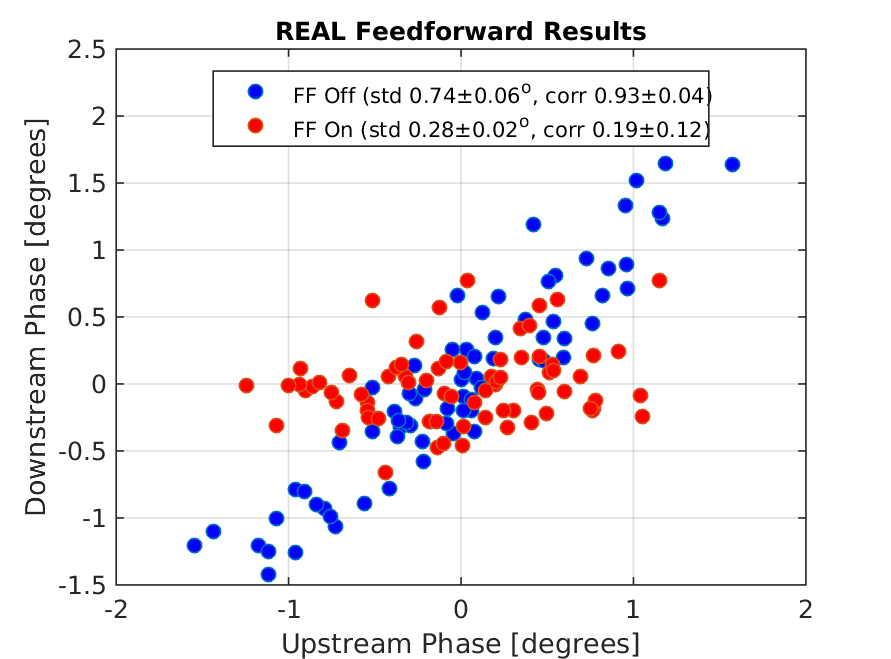
\includegraphics[width=0.45\textwidth]{Figures/feedforward/BestFF_Real}
  \caption{Mean phase.}
  \label{f:BestFF_Real}
\end{figure}

\begin{figure}
  \centering
  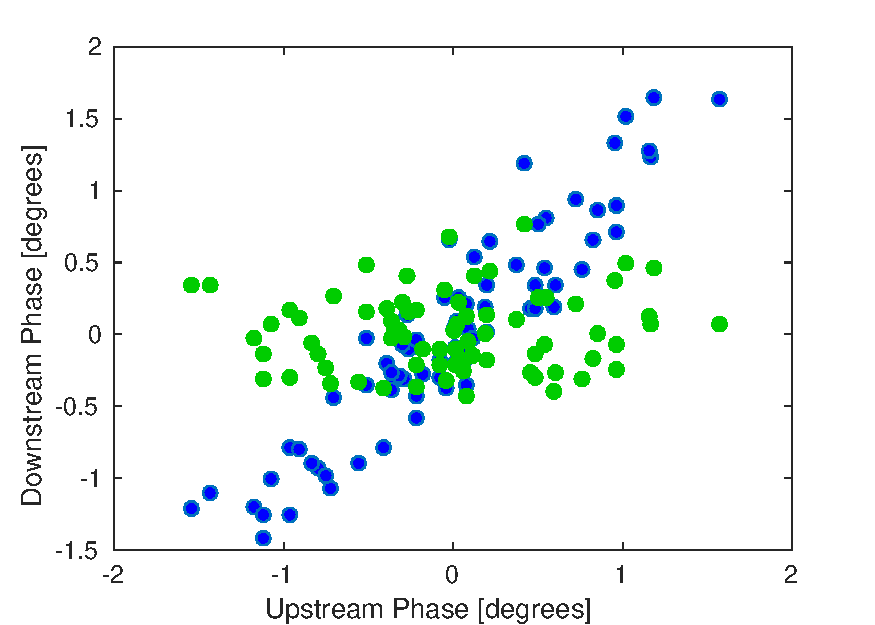
\includegraphics[width=0.45\textwidth]{Figures/feedforward/BestFF_Simulated}
  \caption{Simulated PFF.}
  \label{f:BestFF_Simulated}
\end{figure}


\begin{figure}
  \centering
  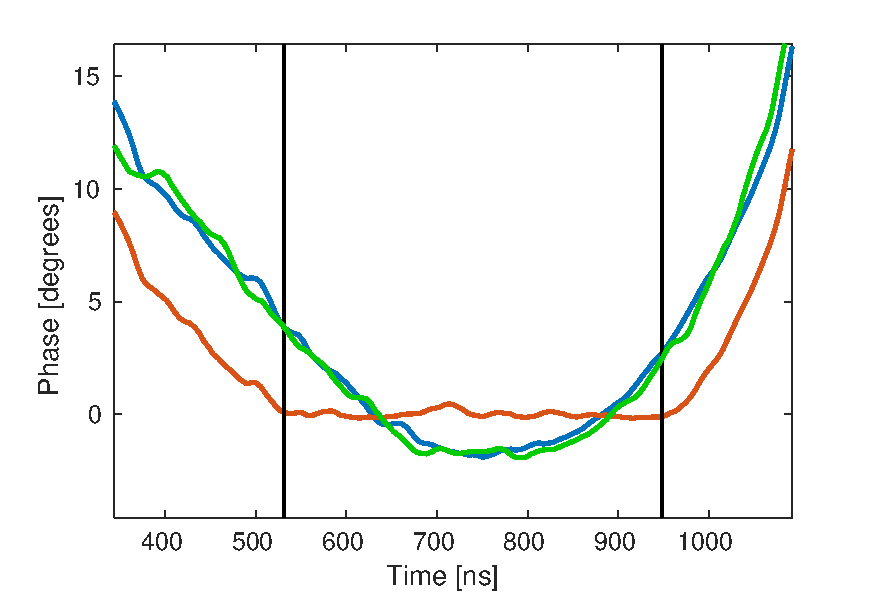
\includegraphics[width=0.45\textwidth]{Figures/feedforward/BestFF_MeanPhaseAlong}
  \caption{Mean phase along.}
  \label{f:BestFF_MeanPhaseAlong}
\end{figure}

\begin{figure}
  \centering
  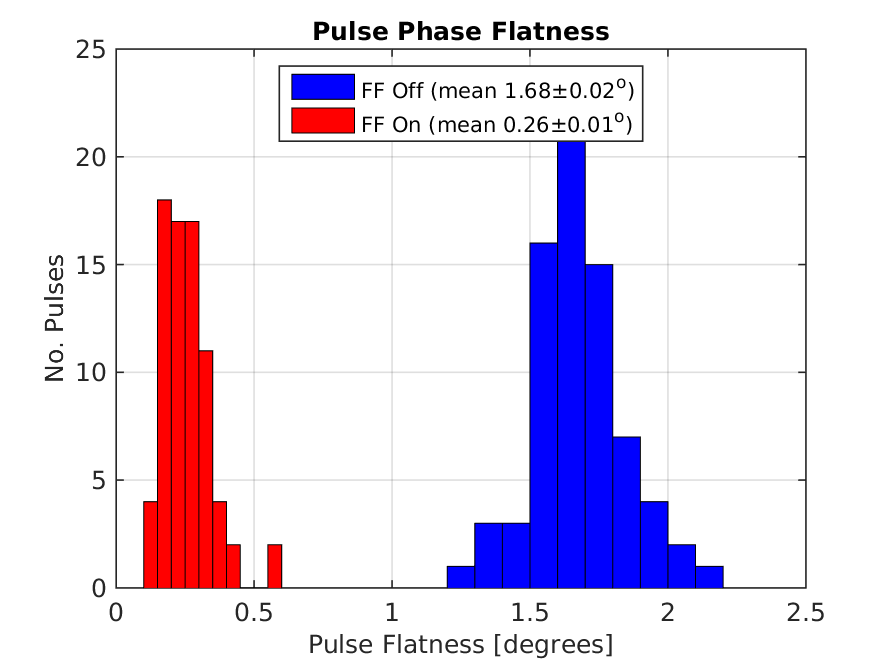
\includegraphics[width=0.45\textwidth]{Figures/feedforward/BestFF_Flatness}
  \caption{Flatness.}
  \label{f:BestFF_Flatness}
\end{figure}

\newsection{longPFF}{Correction on Longer Timescales}

\begin{figure}
  \centering
  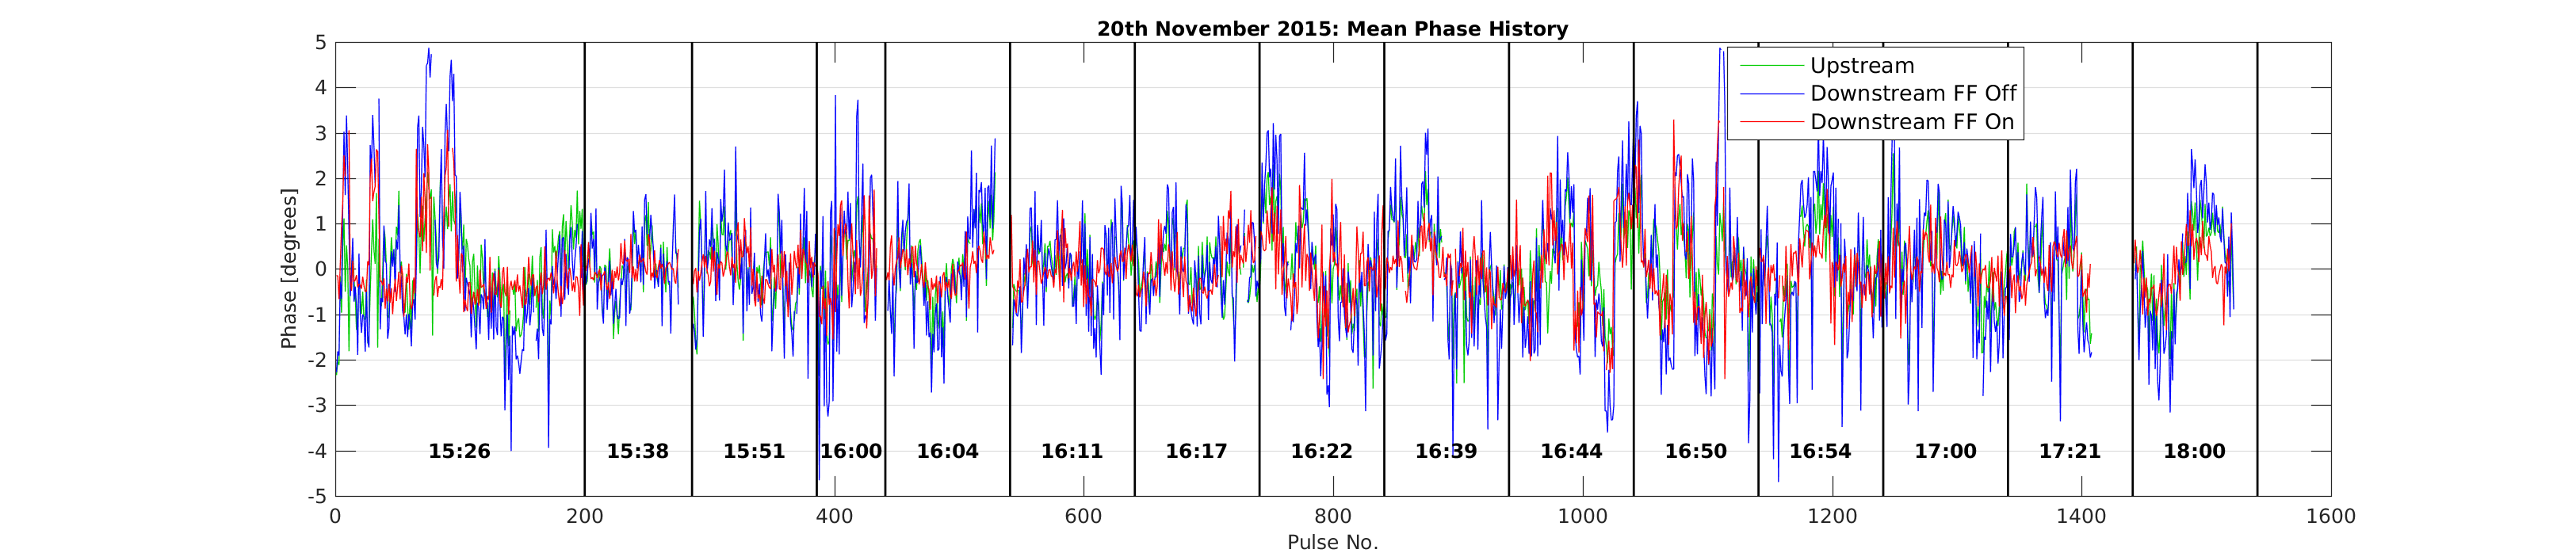
\includegraphics[width=0.45\textwidth]{Figures/feedforward/longFF_history}
  \caption{Flatness.}
  \label{f:longFF_history}
\end{figure}

\begin{figure}
  \centering
  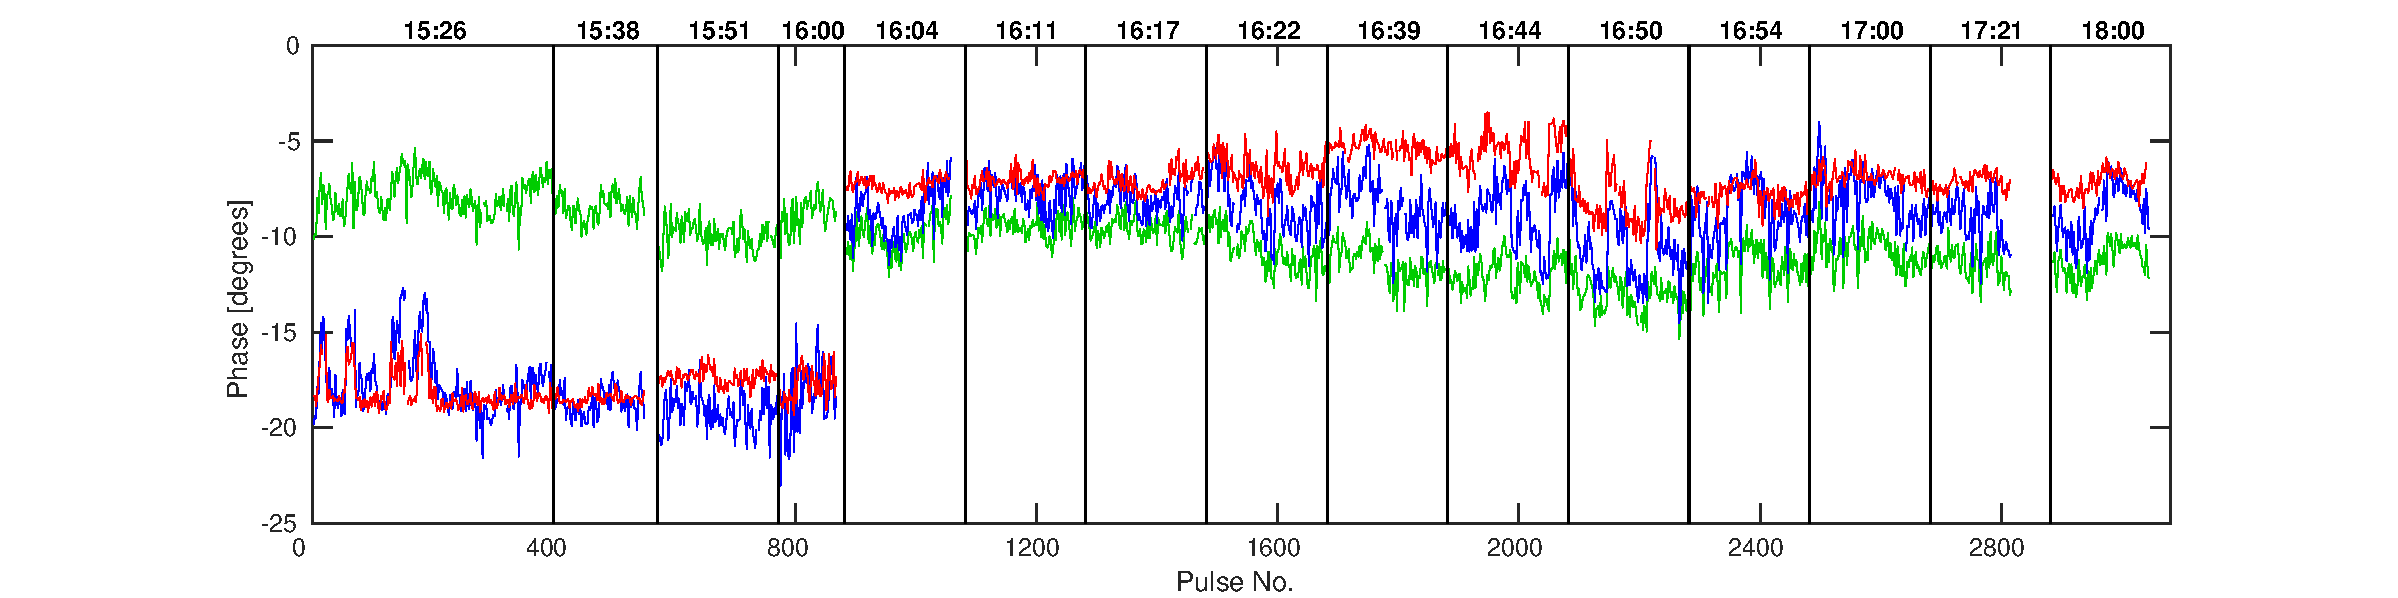
\includegraphics[width=0.45\textwidth]{Figures/feedforward/longFF_noMeanSubHistory}
  \caption{Flatness.}
  \label{f:longFF_noMeanSubHistory}
\end{figure}

\begin{figure}
  \centering
  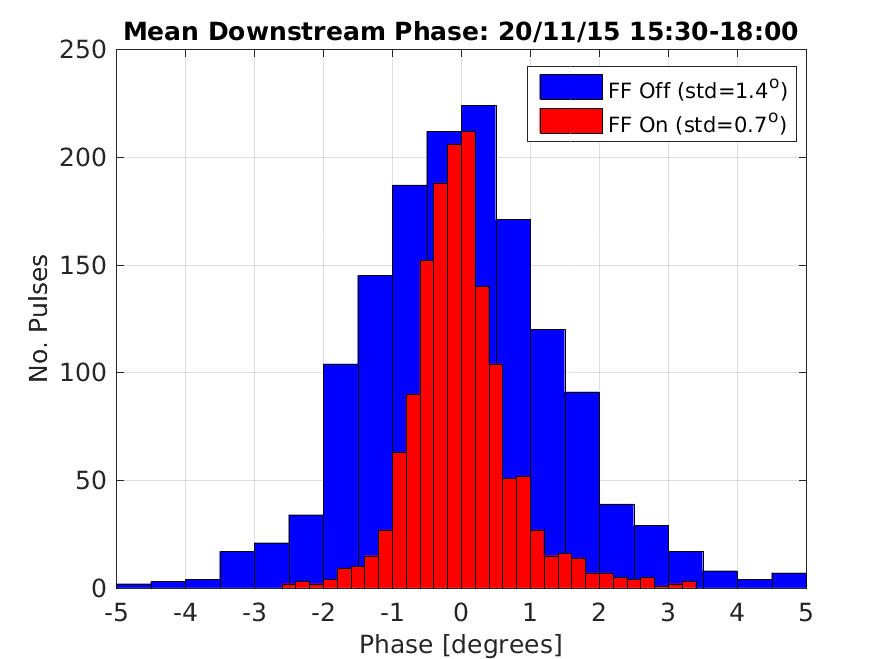
\includegraphics[width=0.45\textwidth]{Figures/feedforward/longFF_histDownstreamPhase}
  \caption{Flatness.}
  \label{f:longFF_histDownstreamPhase}
\end{figure}

\begin{figure}
  \centering
  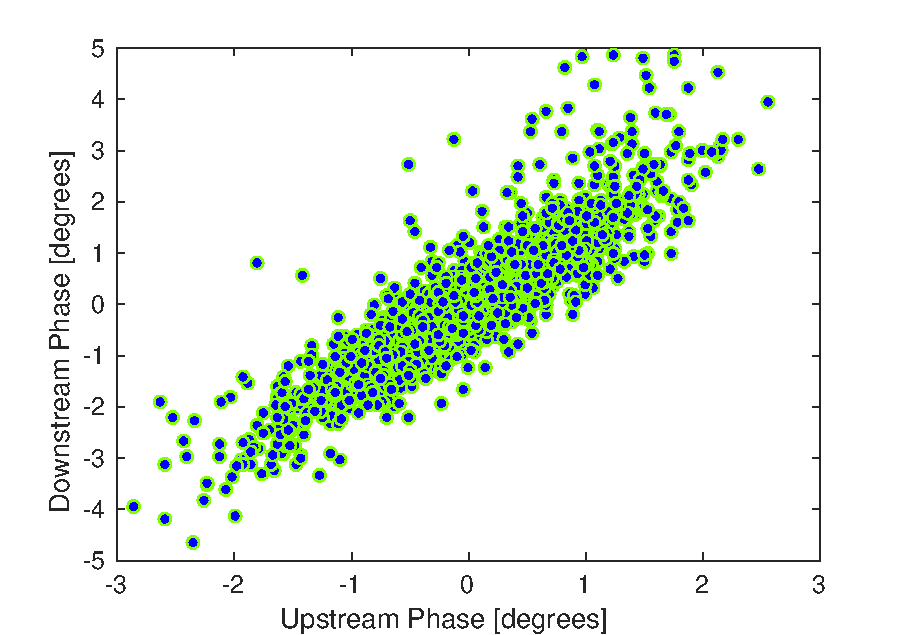
\includegraphics[width=0.45\textwidth]{Figures/feedforward/longFF_scatterFFOff}
  \caption{Flatness.}
  \label{f:longFF_scatterFFOff}
\end{figure}

\begin{figure}
  \centering
  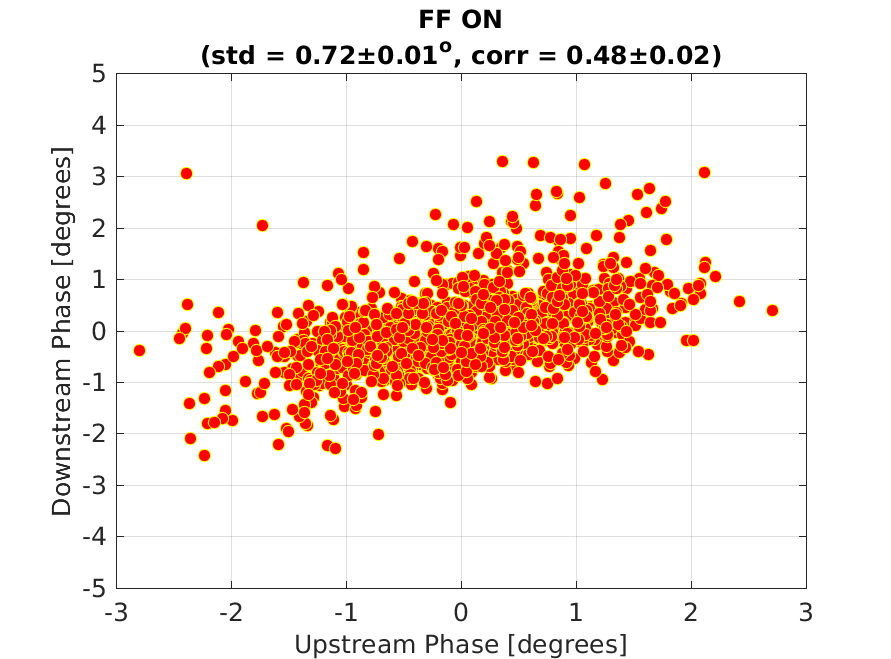
\includegraphics[width=0.45\textwidth]{Figures/feedforward/longFF_scatterFFOn}
  \caption{Flatness.}
  \label{f:longFF_scatterFFOn}
\end{figure}

\begin{figure}
  \centering
  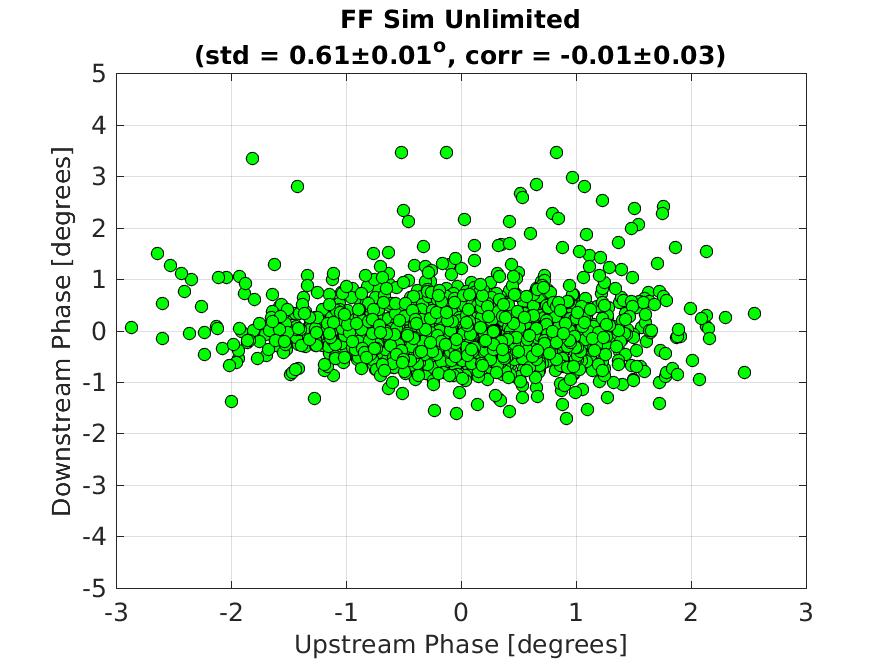
\includegraphics[width=0.45\textwidth]{Figures/feedforward/longFF_scatterFFSimOpt}
  \caption{Flatness.}
  \label{f:longFF_scatterFFSimOpt}
\end{figure}

\begin{figure}
  \centering
  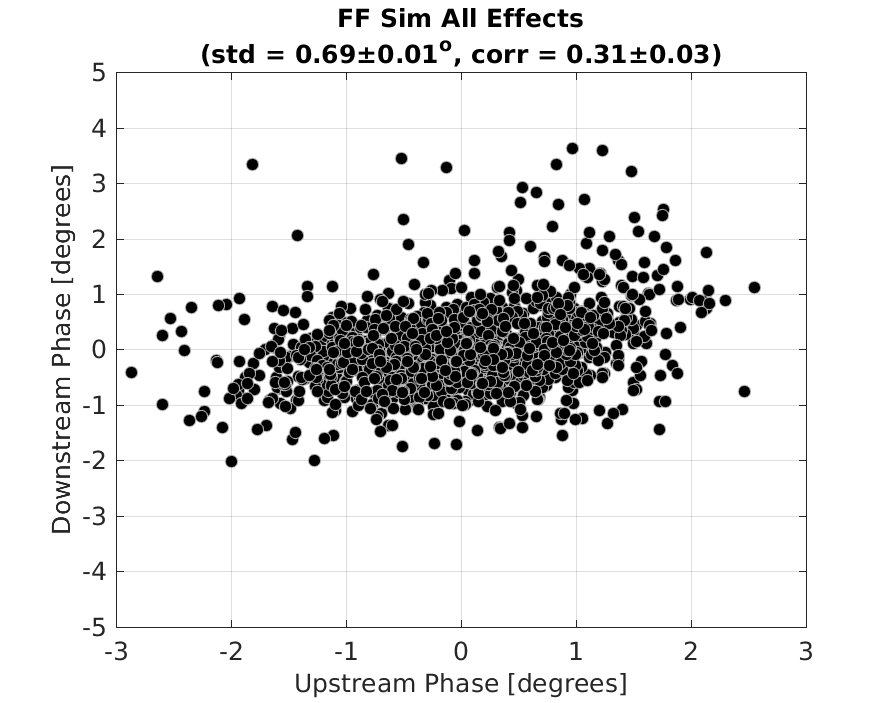
\includegraphics[width=0.45\textwidth]{Figures/feedforward/longFF_scatterFFSimReal}
  \caption{Flatness.}
  \label{f:longFF_scatterFFSimReal}
\end{figure}




\newsection{pffNovelSetups}{Correction with Additional Jitter Source}

At CLIC the PFF system will be required to reduce the initial phase jitter by an order of magnitude, from 2 degrees to 0.2 degrees [REF]. With the initial phase jitter of typically 0.8 degrees at CTF3 it is not possible to demonstrate more than a factor 4 reduction in the jitter using the PFF prototype due to hardware limitations, more specifically due to the achieved phase monitor resolution of 0.14 degrees which limits the theoretical best possible correction to 0.2 degrees \ref{s:resolution}. A secondary goal of the PFF prototype in addition to achieving the baseline goal of 0.2 degrees phase jitter is to demonstrate the factor 10 reduction in jitter relevant to CLIC. In order to do this additional sources of phase jitter must be added.

Clearly, the additional source must be prior to the upstream phase monitor in order to add an additional jitter component that is present in both the upstream and downstream monitors. The correlation between the resulting upstream and downstream phase must be  \(99.5\%\) in order for a factor 10 reduction in jitter to be possible (see Section \ref{ss:theoryJitter}). Two different methods to achieve this have been attempted --- firstly by varying the phases of all the klystrons in the injector and secondly by using the non-zero R56 stretching chicane (see Figure \ref{f:ctfLayout}) at the end of the CTF linac in order to intentionally add an energy component to the upstream phase (which propagates downstream).

\newsection{slowCorr}{Slow Correction}

As the PFF system has only a small range of \(\pm6^{o}\), a secondary ``slow phase feedback" or ``slow correction" has also been implemented at CTF3 to be able to remove larger drifts or static offsets in the downstream phase. In principle this slow correction can be used in conjunction with the PFF system to maximise its performance by keeping the mean uncorrected phase well-centred (zeroed) within its \(\pm6^{o}\) range so that the full power of the PFF amplifiers can be used to correct the fast pulse-to-pulse and intra-pulse phase jitter. If the beam phase were to drift away by \(15^{o}\), for example, the calculated PFF correction would saturate the amplifier across the full pulse length to give the maximal shift of \(6^{o}\). In this case the drift would be partially removed downstream but the PFF system would no longer have any effect on the phase jitter (as the output voltage to the kickers is constant in saturation rather than varying with the phase).

The design and results from the slow correction are discussed in this section. To date its main use has been to verify the ability to shift the beam phase in the TL2 chicane in early-2014 prior to the kicker amplifiers being available to commission the PFF system itself. The slow phase feedback has not yet been used in parallel with the PFF system apart from preliminary tests thus the results shown here are primarily a proof of principle. As PFF attempts have so far been predominantly taken in short datasets of up to a few hundred pulses any large drifts that arise can be manually removed between datasets, either by changing the correction setup (e.g. by changing the phase monitor phase shifters to re-zero the phase) or by re-establishing the previous beam conditions. The slow correction will however be an important tool for future attempts to demonstrate CLIC-level phase stability on time scales longer than a few minutes at CTF3.

\subsection{Implementation}
\label{ss:slowCorrMethod}

Ratio of corrector strengths for orbit closure.

\subsection{Results}
\label{ss:slowCorrResults}




